\documentclass[xcolor=pdftex,dvipsnames,table,mathserif,aspectratio=169]{beamer}
\usetheme{metropolis}
%\usetheme{Darmstadt}
%\usepackage{times}
%\usefonttheme{structurebold}

\usepackage[english]{babel}
%\usepackage[table]{xcolor}
\usepackage{pgf,pgfarrows,pgfnodes,pgfautomata,pgfheaps}
\usepackage{amsmath,amssymb,setspace,outline}
\usepackage{hyperref,url}
\usepackage[latin1]{inputenc}
\usepackage[T1]{fontenc}
\usepackage{relsize}
\DeclareMathSizes{10}{10}{6}{6} 


\title [Single-agent dynamic optimization models]{Single-agent dynamic optimization models}
\author{C.Conlon - help from M. Shum and Paul Scott}
\institute{Grad IO }
\date{}
\setbeamerfont{equation}{size=\tiny}

\begin{document}
\begin{frame}
\titlepage
\end{frame}

\section{Rust Implementation}

\begin{frame}{Rust (1987)}
Likelihood function for a single bus:
\begin{equation*}
\begin{split}
& l (x_1, \cdots , x_T, i_t, \cdots , i_T | x_0, i_0 ; \theta) \\
= & \prod^T_{t=1} Prob (i_t, x_t | x_0, i_0, \cdots , x_{t-1}, i_{t-1} ; \theta) \\
= & \prod^T_{t=1} Prob (i_t, x_t |  x_{t-1}, i_{t-1} ; \theta) \\
= & \prod^T_{t=1} Prob (i_t | x_t; \theta) \cdot \prod^T_{t=1} Prob (x_t | x_{t-1}, i_{t-1} ; \theta_3) .
\end{split}
\end{equation*}
The third line arises from the Markovian feature of the problem, and the last equality arises due to the conditional independence assumption. 
\end{frame}

\begin{frame}{Rust (1987)}
Log likelihood is additively separable in the two components:
\begin{equation*}
\text{log } l(\theta) = \sum^T_{t=1} \text{log } Prob (i_t | x_t ; \theta_1) + \sum^T_{t=1} \text{log } Prob (x_t | x_{t-1}, i_{t-1}; \theta_3).
\end{equation*}
Give the factorization of the likelihood function above, we can estimate in two steps... \\
\vspace{3mm}
\end{frame}

\begin{frame}{Step 1: Estimate Markov TPM}
\footnotesize
\begin{itemize}
\item Estimate $\theta_3$, the parameters of the Markov transition probabilities for mileage, conditional on non-replacement of engine (i.e. $i_t = 0$)
\item Recall that $x_{t+1} = 0$ if $i_t = 1$
\end{itemize}

We assume a discrete distribution for $\triangle x_t \equiv x_{t+1} - x_t$, the incremental mileage between any two periods:
\begin{align*}
\triangle x_t = \left \{ 
\begin{matrix}
[0, 5000) & \text{w/prob } p \\
[5000, 10000) & \text{w/prob } q \\
[10000, \infty) & \text{w/prob } 1 - p - q  
\end{matrix}
\right .
\end{align*}
so that $\theta \equiv \{p, q \}$, with $0 < p, q< 1$ and $p + q < 1$. \\
\vspace{2mm}
\begin{itemize}
\item $\hat \theta_3$ estimated by empirical frequencies: $\hat p = \text{freq} \{ \triangle x_t \in  [0, 5000) \}$, etc. 
\item Note: this does not require the behavioral model!
\end{itemize}
\end{frame}

\begin{frame}{Step \#2: Estimate Structural Parameters of Cost Function}
\footnotesize
Start by treating $(\beta, \hat \theta_3)$ as given:
\begin{enumerate}
\item Fix a guess of $(RC,\theta_1)$ the remaining parameters. 
\item Iterate on the Bellman Operator for $(\beta,\theta_1,\theta_3,RC)$ using \alert{Value Function Iteration} to get $V^*(x,\varepsilon)$ or $\tilde V^*(x,\varepsilon)$.
\item Calculate \alert{conditional choice probabilities} (CCPs):
\begin{align*}
Pr(i_t=1 | x_t,\varepsilon_t,\theta) &=  \frac {\exp[ \tilde V_{\theta} (x_t, \varepsilon_t, 1)]  }{\exp[\tilde  V_{\theta} (x_t, \varepsilon_t, 0)] + \exp[ \tilde  V_{\theta} (x_t, \varepsilon_t, 1)]} 
\end{align*} 
\item Evaluate the log-likelihood:
\begin{align*}
\log l(\theta) = \sum^T_{t=1} \log \text{Pr} (i_t | x_t ; \theta_1,RC) + \underbrace{\sum^T_{t=1} \log \text{Pr} (x_t | x_{t-1}, i_{t-1}; \hat{\theta}_3)}_{\text{Can Ignore! Why?}}
\end{align*}
\end{enumerate}
Solve via MLE. This is the \alert{Nested Fixed Point} algorithm.
\end{frame}

\begin{frame}{Computational Details}
That looked easy, except that I never really showed you how to recover $\tilde{V}_{\theta}(x,i)$:
\begin{itemize}
\item Directly iterating on Bellman's operator requires keeping track of $\varepsilon$'s which are: (1) unobserved to you the econometrician and (2) continuous and full support (not a discrete grid).
\begin{itemize}
\item AKA a big pain.
\end{itemize}
\item You may (or may not) have learned some tricks for solving Bellman equations in Macro that you could apply here: VFI, Policy Iteration (PI), Howard's Policy Improvement, etc.
\begin{itemize}
\item None of that really tells us how to deal with $\varepsilon$'s.
\end{itemize}
\end{itemize}
\end{frame}

\begin{frame}{Rust's Trick}\

\begin{itemize}
\item Rust has a nice trick that let's us work with a new function $EV_{\theta}(x,i)$ instead of $V_{\theta}(x,i,\varepsilon)$ we call this the \alert{ex ante} or \alert{expected value function}.
\begin{eqnarray*}
EV(x, i) \equiv E_{x', \varepsilon ' | x, i} V(x', \varepsilon ' ; \theta)
\end{eqnarray*}
\item In words $EV_{\theta}(x,i)$ says at time $t-1$ what is the expected value of $V_{\theta}(x_t,\varepsilon_t)$ [eq 4.14].
\begin{eqnarray*}
\resizebox{.9\hsize}{!}{$EV(x,i) = \int_y \log \left \{ \sum_{j \in C(y)} \exp [ u(y,j; \theta) + \beta EV(y, j)] \right \} p(dy|x,i) $}
\end{eqnarray*}
\item Here $x, i$ denotes the \emph{previous} period's mileage and replacement choice, and $y, j$ denote the \emph{current} period's mileage and choice. 
\end{itemize}
\end{frame}

\begin{frame}{Derivation of Rust's Trick}
\footnotesize
This \alert{ex ante value function} can be derived from Bellman's equation:
\begin{align*}
\begin{split}
V(y, \varepsilon ;\theta) = & \max_{j \in 0,1} [ u(y, j ; \theta) + \varepsilon_j + \beta EV(y,j)] \\
\Longrightarrow & E_{y, \varepsilon} [V(y, \varepsilon ; \theta) | x, i ] \equiv  EV(x, i ; \theta) \\
= & E_{y, \varepsilon | x, i } \left \{ \max_{ j \in 0,1} [ u(y, j ; \theta) + \varepsilon_j + \beta EV(y,j)] \right \} \\
= &  E_{y | x, i }  E_{\varepsilon | x, i } \left \{ \max_{ j \in 0,1} [ u(y, j ; \theta) + \varepsilon_j + \beta EV(y,j)] \right \} \\
= &  E_{y | x, i } \log \left \{ \sum_{j=0,1} \exp [ u(y, j ; \theta)  + \beta EV(y,j)] \right \} \\
= & \int_y \log  \left \{ \sum_{j=0,1} \exp [ u(y, j ; \theta)  + \beta EV(y,j)] \right \} p(dy|x,i).
\end{split}
\end{align*}
\end{frame}
%
%\begin{frame}{Rust (1987)}
%The next-to-last equality uses the closed-form expression for the expectation of the maximum, for extreme-value variates.\\
%\vspace{3mm}
%Once the $EV(x, i ;\theta)$ function is computed for $\theta$, the choice probabilities $p(i_t |x_t)$ can be constructed as
%\begin{equation*}
%\frac {\exp(u(x_t, i_t ;\theta) + \beta EV (x_t, i_t; \theta))}{\sum_{i=0,1} \exp(u(x_t, i;\theta) + \beta EV(x_t, i;\theta))}.
%\end{equation*}
%\end{frame}

\begin{frame}{Value Function Iteration}
\footnotesize
\begin{enumerate}
\item Start with an initial guess at $\tau=0$ for $EV^{\tau}_{\theta}(x,i)$. A common guess is $EV_{\theta}^{\tau}(x,i) = 0$ for all $(x,i)$
\item Iterate Bellman Operator
\begin{align*}
T_{\theta}\left(EV_{\theta}^{\tau}\right)= & \int_y \log  \left \{ \sum_{j=0,1} \exp [ u(y, j ; \theta)  + \beta EV^{\tau}(y,j)] \right \} p(dy|x,i).
\end{align*}
with $p(dy | x, i; \hat \theta_3)$ estimated in Step 1.\\

$T_{\theta}\left(EV_{\theta}^{\tau}(x,i)\right)\equiv EV_{\theta}^{\tau+1}(x,i)$.\\
\item Compare $\epsilon(\tau) \equiv \sup_{(x,i)} | EV_{\theta}^{\tau+1}(x,i) - EV_{\theta}^{\tau}(x,i)|$ to $\epsilon^{tol}$. If $\epsilon(\tau) \leq \epsilon^{tol}$ then stop.
\end{enumerate}
See my notes on Numerical Dynamic Programming for more details.
\end{frame}

\begin{frame}{Solving the fixed point}
Obvious approach is contraction iterations (VFI):
\begin{align*}
E V_{\theta}^{\tau}=T_{\theta}\left(E V_{\theta}^{\tau-1}\right)=T_{\theta}^{\tau}\left(E V_{0}\right)
\end{align*}
Rust actually switches to Newton-Kantorovich Iteration:
\begin{align*}
E V_{\theta}^{\tau+1}=E V_{\theta}^{\tau}-\left[I-T_{\theta}^{\prime}\right]^{-1}\left(I-T_{\theta}\right)\left(E V_{\theta}^{\tau}\right)
\end{align*}
The first is slow, but globally convergent. The second is fast but locally convergent. To get the gradient of the log-likelihood we must also calculate the Jacobian using the IFT:
\begin{align*}
\partial E V_{\theta} / \partial \theta=\left[I-T_{\theta}^{\prime}\right]^{-1} \partial T_{\theta}\left(E V_{\theta}\right) / \partial \theta
\end{align*}
See \url{https://editorialexpress.com/jrust/nfxp.pdf} for more details.
\end{frame}



\begin{frame}{Value Function Iteration: Bounds}
\begin{itemize}
\item Suppose we set $V_0 =0$ then the value function iteration approach is just like solving the finite horizon problem by backward induction.
\item The CMT guarantees consistency at a geometric rate or \alert{linear} convergence with modulus $\beta$
\item We can derive an expression for the number of steps we need to get an $\epsilon$-approximation.
\begin{eqnarray*}
T(\epsilon,\beta) = \frac{1}{| \log(\beta) | } \log \left (\frac{1}{(1-\beta)\epsilon} \right)
\end{eqnarray*}
\item This tells us that when $\beta \rightarrow 1$ that VFI gets very very slow.
\end{itemize}
\end{frame}



\begin{frame}{Estimates}
\begin{center}
\hspace*{-.5cm}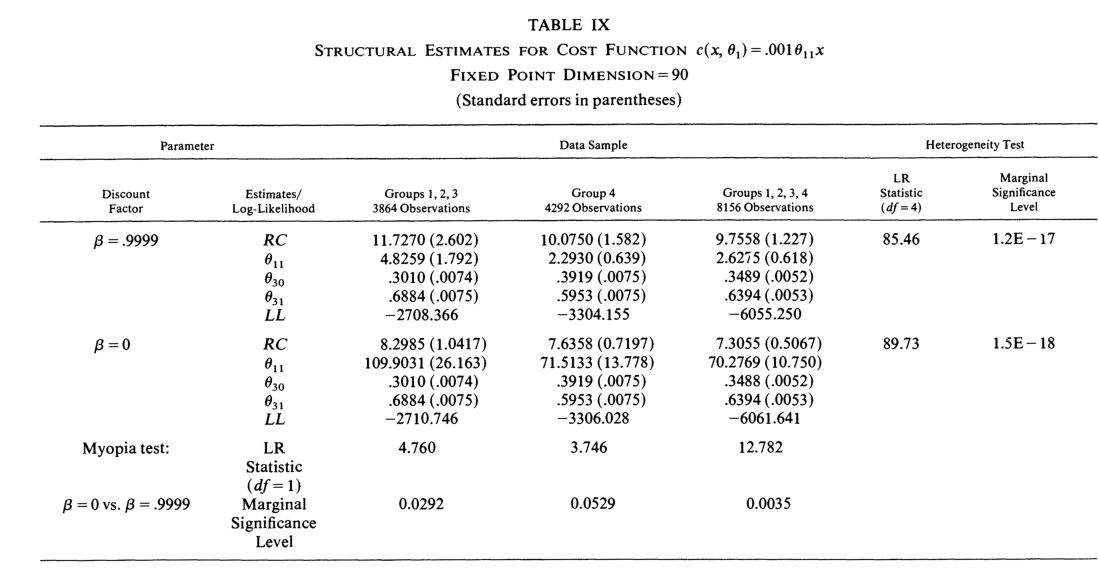
\includegraphics[scale=.65]{./resources/RustT9.pdf}
\end{center}
\end{frame}

\begin{frame}{Discount factor}
\begin{itemize}
	\item While Rust finds a better fit for $\beta=.9999$ than $\beta=0$, he finds that high levels
	of $\beta$ basically lead to the same level of the likelihood function.

	\medskip
	\item Furthermore, the discount factor is non-parametrically non-identified. Note:
	He loses ability to reject $\beta=0$ for more flexible cost function specifications.

\end{itemize}
\end{frame}


\begin{frame}{Discount factor}
\begin{center}
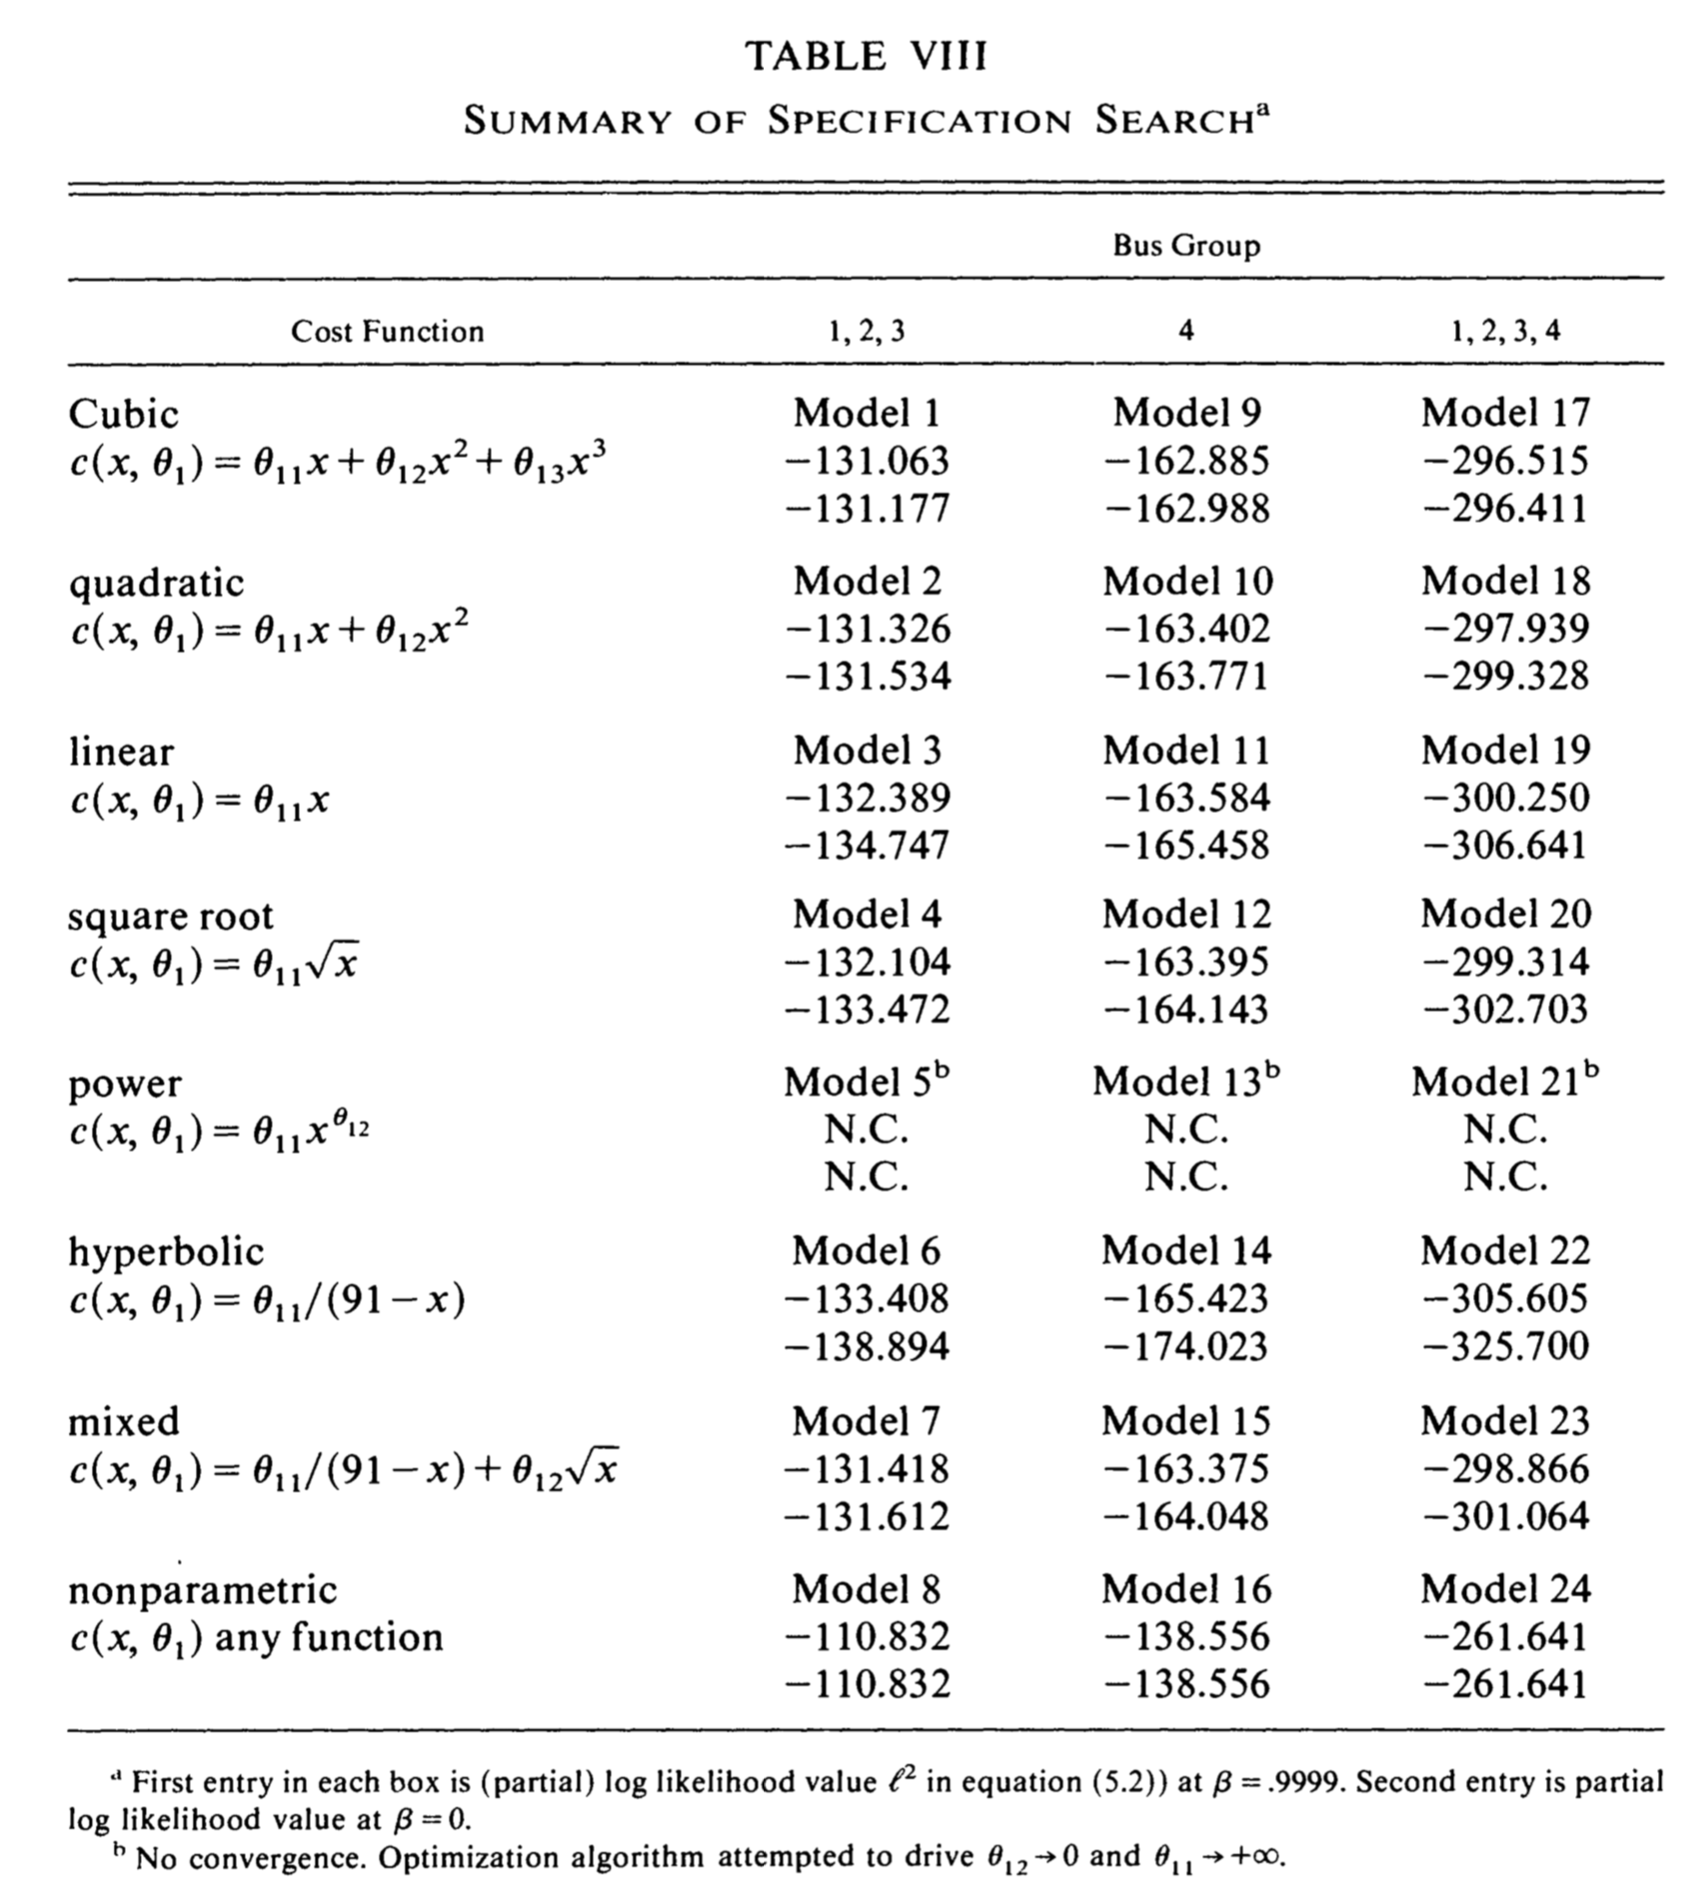
\includegraphics[scale=.25]{./resources/RustT8.png}
\end{center}
\end{frame}

\begin{frame}{Application}
\begin{center}
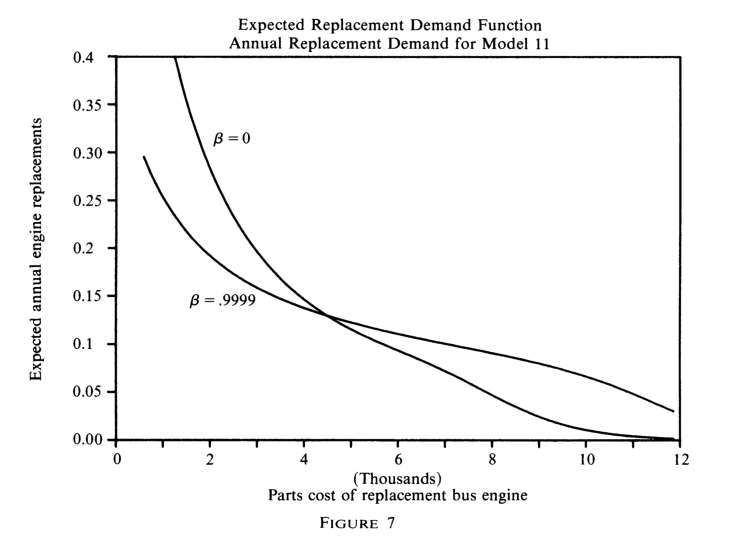
\includegraphics[scale=.8]{./resources/RustF7.pdf}
\end{center}
\end{frame}


\end{document}